%% chapter 5 Metabolic  rates and energetic requirements

\section*{Keywords}
Land use; land-use intensity; metabolic rates; energetic constraints; energetic requirements; terrestrial vertebrates; trophic group; occurrence.

\section*{Abstract}
Land-use change is the primary driver of global biodiversity loss. In terrestrial vertebrates, previous work has shown that sensitivity to land-use change depends on species traits, but the extent to which energetic constraints explain species responses to disturbed land uses remains largely unexplored. Here, I investigate relationships between the energetic requirements of terrestrial vertebrates (estimated from resting metabolic rates) and land-use change, at two levels of organisation. First, at the assemblage level I hypothesize that total energetic requirements in disturbed land uses are lower than in undisturbed land uses, assuming that there is less energy available in these areas overall. Second, after controlling for the effects of body mass and taxonomy on metabolic rates, I predict that species with relatively lower energetic expenditure are favoured over species with relatively higher energetic expenditure in disturbed land uses, as resource efficiency will be beneficial in these resource-poor environments. Because trophic group   influences species ability to assimilate various types of food, I investigate whether my predictions are consistent among trophic groups (here, omnivores, carnivores or herbivores).
The results challenged both hypotheses. I found that total assemblage-level energetic requirements did not systematically decrease in disturbed land uses. For instance, I detected significant increases for urban areas in all trophic groups, highlighting that disturbed areas may not be as energy-poor as I initially assumed. Second, I found a positive effect of metabolic rates (after controlling for body mass and taxonomy) on species probability of occurrence across all trophic groups for at least one of the most disturbed land uses I considered (pasture, cropland and urban). Species for which there are exploitable resources in disturbed environments may benefit from having larger energetic expenditure: they may display a set of characteristics rendering them more able to cope with disturbances and more able to acquire available resources, such as higher activity levels or bigger brain sizes. The findings of this Chapter highlight that land-use change has  substantial impacts on vertebrate community metabolism.   


\section{Introduction}
  
Land-use change is currently the strongest driver of global biodiversity declines \citep{Newbold2015, Maxwell2016}, with major and long-lasting impacts on the structure and functioning of ecological communities \citep{Bregman2016, Fukasawa2019, Magioli2021, Marcacci2021}. With land-use change likely to continue to intensify \citep{Stehfest2019}, it is vital to put into place conservation and mitigation measures to minimise future losses of biodiversity and negative impacts on ecosystem functioning. To this end, pressing questions remain as to what renders species able or unable to cope with human disturbance, and how losses of sensitive species might influence ecosystem functioning \citep{Dirzo2014, Young2016}.    

Land-use change acts as an environmental filter affecting species persistence \citep{Evans2018, Edwards2021}. Past studies have shown that sensitivity to land-use change is distributed unevenly across the tree of life \citep{Nowakowski2018a}, and across behavioural \citep{Lowry2013, Samia2015} and ecological strategies \citep{Newbold2013, Moller2009, DePalma2015}. For instance, long-lived and large forest specialist birds respond more negatively to land-use change than generalist species \citep{Newbold2013}. In addition, human land uses impose energetic constraints on species, by modifying the amount and type of available resources \citep{Inger2016, ZunigaPalacios2021}. Consequently, land-use change brings about modifications in dietary and foraging strategies \citep{Moller2009, Ramesh2017, Seveque2020}, which can have cascading effects on local trophic structure (e.g., mesopredator release; \citet{Crooks2010}). The impacts of land-use change on biodiversity also depend on land-use intensity \citep{Newbold2015, Davison2021}, that is, the magnitude of human disturbance in a given land-use type, which can vary importantly according to local practices and management \citep{Dullinger2021}. In particular, land-use intensity affects the types and availability of resources (by homogenising resources for example), which in turn may affect biodiversity patterns \citep{Weiner2011}.

Energetic requirements are likely to be important predictors of species’ ability to cope with a disturbed environment where resource availability and resource types are strongly impacted \citep{Auer2020}. Past research has shown that metabolic rates (the amount of energy required for organismal maintenance and for other processes such as growth and reproduction) are heritable and subject to selection, for instance with species in energy-rich environments having evolved faster metabolic rates than species in less energy-rich environments \citep{Mueller2001}. However, metabolic rates have received less attention than other life-history traits in studies aiming to understand different species’ responses to land-use change. Body mass, known to explain much of the variation in metabolic rates \citep{White2003, Hudson2013, Bushuev2018}, has been considered in past studies examining effects of land-use disturbance on assemblage composition \citep{Hevia2017}. Since metabolic rates correlate positively with body mass, the effects of land-use change on local energetic requirements have been indirectly assessed through investigations of changes in body mass composition along land-use gradients \citep{Newbold2020a, Tinoco2018}. However, to the best of our knowledge, no study has yet directly reported the effects of land-use change on assemblage-level energetic requirements. 

Thus, the first objective of this Chapter is to investigate how land-use change impacts assemblage-level energetic requirements in terrestrial vertebrates. To this end, I use metabolic rates as a proxy for maintenance energetic requirements at the species level. I predict that, at the assemblage level, total energetic requirements in disturbed land uses are lower than in undisturbed land uses. This prediction relies on the assumption that there is less energy available overall in disturbed land uses than in undisturbed land uses (Figure \ref{chap5_fig1}c), with disturbed land uses being characterised by human appropriation of net primary productivity \citep{Krausmann2013}. Because species’ ability to exploit particular resources and meet energetic demands also depends on food types and diet \citep{Mendoza2019, McNab1986}, I test whether this prediction holds true within trophic groups (i.e., within herbivores, omnivores, and carnivores). Here, I consider energetic requirements at the assemblage level, not controlling for species body mass, to obtain estimates of total energy expenditure in different land-use types \textbf{(Fig. 2a)}. Thus, any changes in assemblage-level energetic requirements could be ultimately driven by shifts in the size-spectrum of local assemblages. 

Body mass explains much of the variation in metabolic rates, but species with similar body masses still display important variation in metabolic rates \citep{Mueller2001}. Some of this variation can be explained by taxonomic position (which also accounts for differences in thermoregulatory strategy between endotherms and ectotherms). However, there remains substantial interspecific variation in metabolic rates even after accounting for body mass and taxonomic affiliation \citep{Mueller2001, White2013}. Food availability and food type might explain this residual variation in metabolic rates among species \citep{Mueller2001}. Species that evolved in areas with abundant resources assimilate and burn calories at high rates, regardless of their body mass -- while species that evolved with limiting resources could process resources at lower rates, irrespectively of their body mass \citep{Mueller2001}. Building upon this idea and the `allocation' principle (i.e., the trade-offs in resource allocation; \citet{Auer2020}), species with lower energetic expenditure (than expected from body mass and taxonomy) may be able to cope with food scarcity better than those with larger energy expenditure (than expected from body mass and taxonomy). Indeed, regardless of their body mass, such species should need fewer resources to meet energetic demands \citep{Clarke2004a}. Thus, as land-use disturbance modifies the types and abundance of resources, we expect species energetic requirements --after removing the effects of body mass and taxonomic position-- to influence responses to land-use change. Yet, whether energetic constraints explain species responses to land-use change in terrestrial vertebrates has not been investigated before \citep{Hevia2017}. Thus, the second objective of this Chapter is to characterise the influence of energetic constraints on species occurrence probability in disturbed land uses, compared to undisturbed land uses. I approximate energetic constraints at the species level from residual variation in metabolic rates, that is, the variation not explained by body mass or taxonomy. I predict that species with negative deviations (lower rates than expected from body mass and taxonomy) are more likely to persist in disturbed land uses than species with positive deviations (higher rates than expected from body mass and taxonomy; \textbf{Fig. 2b}). Given that trophic group can influence resource acquisition and species ability to assimilate various types of food, I investigate whether this prediction is consistent among trophic groups.

To test both predictions, I use a space-for-time substitution approach, obtaining vertebrate assemblage composition data from the PREDICTS database \citep{Hudson2014, Hudson2017}. I combine this database with trophic-group information (characterising species as either omnivores, herbivores, or carnivores), and with species-level estimates of resting metabolic rates and body mass. 
  
\begin{figure}[h!]
\centering
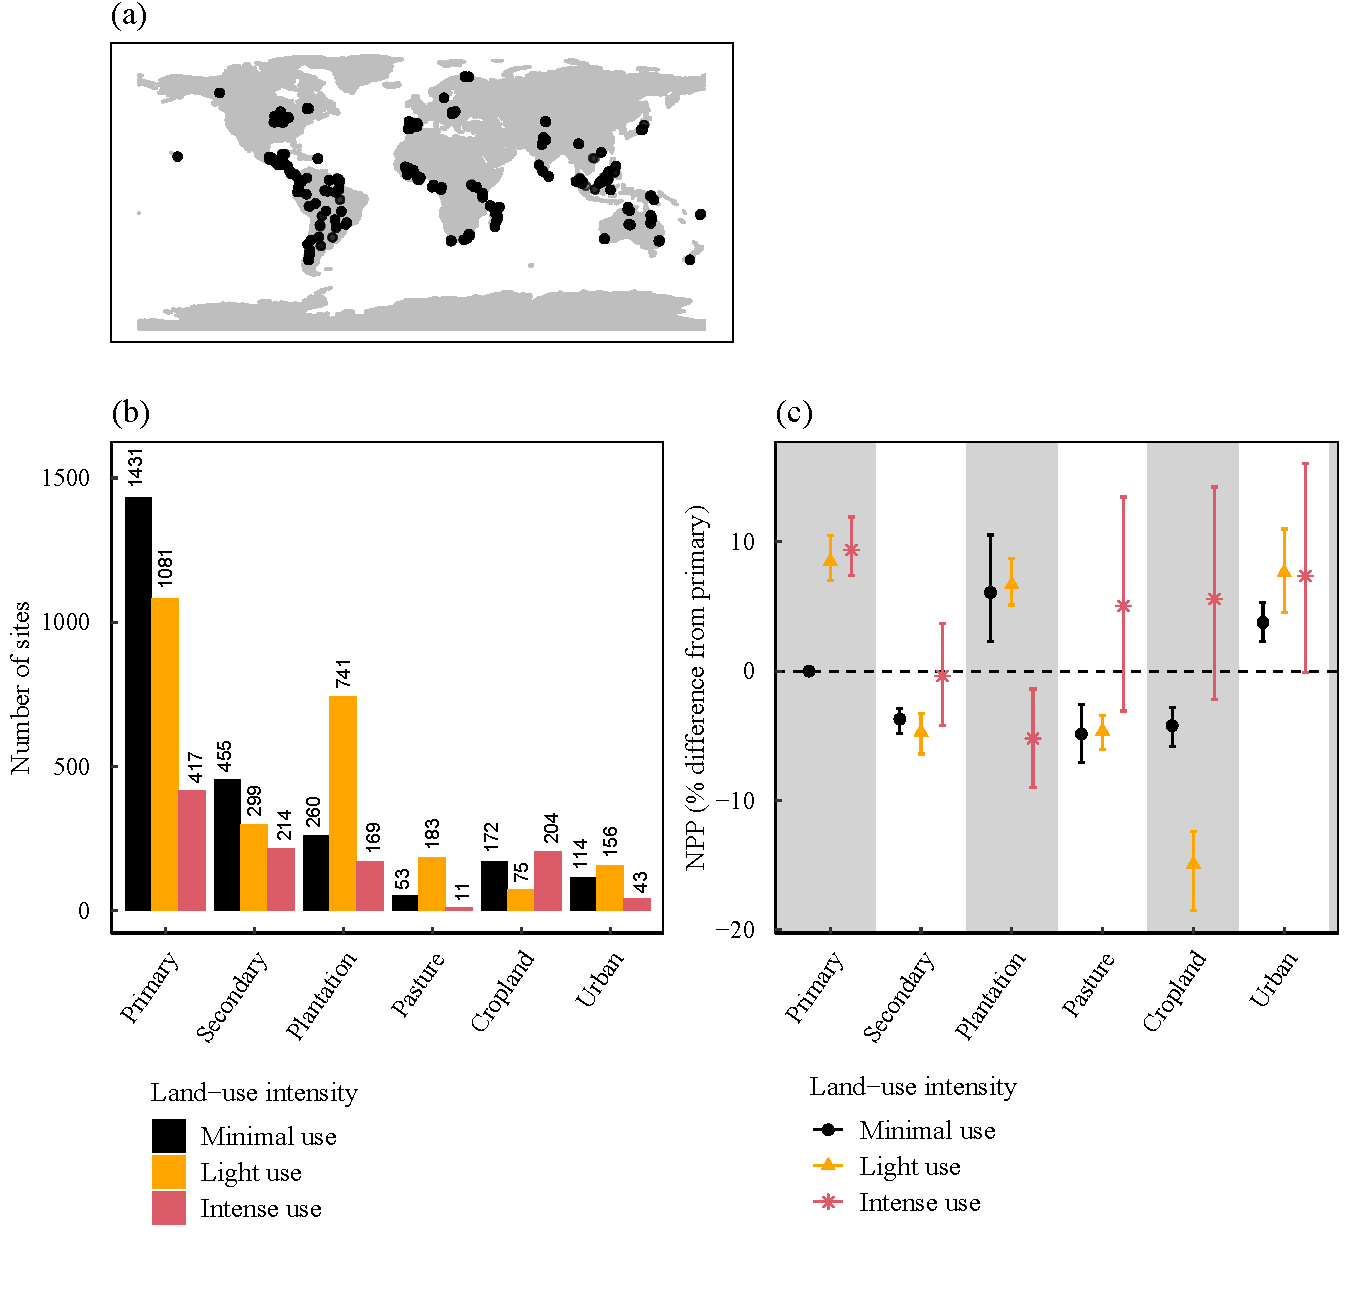
\includegraphics[scale=0.75]{figures/Chapter5/Figure1}
\caption[Map of PREDICTS sites, sample sizes and NPP by land use and land-use intensity]{\textbf{(a) Spatial distribution of the sampled sites} from the PREDICTS database for terrestrial vertebrates (6,484 sites); (\textbf{b) Number of sites in each land-use and land-use-intensity category;} \textbf{(c) Net primary productivity by land use and land-use intensity} (derived from MODIS satellite imagery), with model predictions plotted relative to minimally used primary vegetation (and rescaled with reference to that land-use type). Primary: primary vegetation; secondary: secondary vegetation; plantation: plantation forest.}
\label{chap5_fig1}
\end{figure}

\section{Methods}

\subsection{Vertebrate assemblage composition }

I obtained vertebrate assemblage composition in different land uses from the PREDICTS database \citep{Hudson2014, Hudson2017}. The PREDICTS database is a large collection of published studies that measure biodiversity across different land uses and is one of the most comprehensive global databases of its type. In each PREDICTS study, species occurrence and often abundance were recorded across different sites. Each site was assigned to one of the following land-use types: primary vegetation (natural, undisturbed vegetation), secondary vegetation (recovering after complete destruction of primary vegetation), plantation forest (woody crops), pasture (areas grazed by livestock), cropland (herbaceous crops) and urban (built-up areas). The land-use categories were assigned based on habitat descriptions from the original studies \citep{Hudson2014}, sometimes in consultation with the original study authors. Each site was also classified in terms of land-use intensity as either minimal, light or intense. The land-use-intensity assignment was also made on the basis of the habitat description in the original studies, and depended on criteria specific to each land use (such as degree of mechanisation, yield or chemical inputs for cropland; or the amount of green space in urban areas; \citet{Hudson2014}).  

I subset the PREDICTS database for studies that sampled terrestrial vertebrates, and for which both land use and land-use intensity had been characterised. I thus obtained 181 studies for 4,238 species sampled across 6,484 sites (Figure \ref{chap5_fig1}a). Sample sizes varied across land uses and land-use intensities (Figure \ref{chap5_fig1}b). 

\subsection{Energy availability by land-use type and land-use intensity}

The predictions of this Chapter rely on the assumption that resource types and abundance are modified in disturbed environments, with less energy available in disturbed compared to undisturbed land uses overall. To test this assumption, I used terrestrial net primary productivity (NPP) across land uses as a proxy for available energy. NPP quantifies the amount of atmospheric carbon fixed by plants and accumulated as biomass. NPP estimates were derived using imagery from the Moderate Resolution Imaging Spectroradiometer (MODIS) on board NASA’s Terra satellite. NPP estimates were based on a yearly composite of measures made at 8-day intervals, captured at 500-m spatial resolution \citep{Running2015}. I obtained NPP for 4,062 of the PREDICTS sites used in the analysis (matching the sites to the NPP data using the sampling year available in PREDICTS). I fit a linear mixed-effects model (lme4 package, version 1.1-23, \citet{Bates2015}) explaining site-level NPP by land use and land-use intensity, with a random intercept accounting for study identity, to control for differences in experimental design across studies. Model predictions showed that NPP decreased significantly in several land uses (e.g., pasture and cropland) compared with the primary vegetation reference level, although the strength and in some cases direction of the difference varied among land-use and land-use intensity combinations (e.g., increases in urban land uses; Figure \ref{chap5_fig1}c).

\subsection{Resting Metabolic Rates (RMR) \& imputations of missing RMR values}

As a proxy for species-level energetic expenditure, I used estimates of the minimum amount of energy required for organismal maintenance, i.e., basal metabolic rates (BMR) for endotherms, and resting metabolic rates (RMR) for ectotherms. From the literature, I obtained estimates of BMR for 719 species of birds and 685 mammals, and estimates of RMR for 126 amphibians and 173 reptiles (\textbf{Supporting information, Table S1}). For endotherms, BMR are measured when species are in their thermoneutral zone, that is, when there is little to no energy expenditure allocated to thermoregulation. Thus, BMR estimates were derived from lab studies that mostly measured oxygen consumption of the organisms at rest under controlled conditions and in the thermoneutral zone of the species. For an ectotherm, there is no `basal' metabolic rate, as body temperature mainly depends on environmental temperature. Their metabolic rates follow a hump-shaped relationship with environmental temperature, highest at an optimal temperature which corresponds to a performance peak. To be able to compare endotherms’ BMR with ectotherms’ RMR, \citet{Stark2020} used the metabolic rates that correspond to a performance peak for both groups (i.e., BMR in the thermoneutral zone for endotherms, and metabolic rates at optimal temperature for ectotherms). Thus, I used the data compiled in \citet{Stark2020} for ectotherms, and from the sources specified in \textbf{Table S1} for endotherms. The units for BMR and RMR were standardized to mL of dioxygen consumed per hour (mLO$_2$/h). As in \citet{Stark2020}, I henceforth refer to both basal and resting metabolic rates as RMR. 

For the species occurring in PREDICTS, initial data coverage for RMR was poor (\textbf{Table S1}), necessitating imputation of missing values. To do so, I first measured the phylogenetic signal in BMR and RMR (log$_e$-transformed), using Pagel’s $\lambda$ \citep{Pagel1999}, to assess whether metabolic rates were sufficiently phylogenetically conserved to be estimated from species phylogenetic position. I obtained class-specific phylogenetic trees from \citet{Jetz2012} for birds, from \citet{Faurby2018, Faurby2020} for mammals, from \citep{Tonini2016} for reptiles (squamates), and from \citet{Jetz2018} for amphibians (all downloaded in April 2020). For each class, I randomly sampled 100 trees. To account for phylogenetic uncertainty, I calculated Pagel’s $\lambda$ for each sampled tree and reported the median value, as well as the 2.5th and 97.5th percentiles (\textbf{Table S1}).  

In addition to being highly phylogenetically conserved \textbf{(Table S1)}, RMR correlate strongly with body mass \textbf{(Fig. 2a)}. Thus, I imputed missing values using body-mass information (see next section), phylogenetic relationships and taxonomic orders as predictors \citep{Penone2014}. For each class, I used a consensus phylogenetic tree from which I summarised phylogenetic relationships in the form of five phylogenetic eigenvectors. Including more eigenvectors had little impact on the imputed values (results not shown). 
\begin{comment} For instance, after re-imputing the values using 10 eigenvectors, the correlation coefficient between the values imputed with 5 eigenvectors and with 10 eigenvectors was 0.997, showing high levels of congruence between the imputed values, regardless of the number of eigenvectors). 
\end{comment}
Consensus trees were obtained with the TreeAnnotator programme of the BEAST software \citep{Bouckaert2014}. Missing RMR values were imputed using random forests algorithms implemented in R using the ‘missForest’ package (version 1.4; \citet{Stekhoven2012, Stekhoven2016}).  

\subsection{Trophic group and body mass information}

I used body mass and trophic group information for terrestrial vertebrates compiled in Chapter 2. Body mass was compiled as a single measure at the species level, meaning I was unable to consider intraspecific variation. Trophic group described species as either carnivores, omnivores, or herbivores. Because there were gaps in the availability of the data, more so for trophic group than for body mass (see Chapter 2), I imputed the missing trait values (independently of RMR imputations), then used both imputed and empirical body mass values for imputations of missing RMR values. To impute missing body mass and trophic groups, I used random forests algorithms (again, using the missForest R package), including as additional predictors phylogenetic information, added in the form of 10 phylogenetic eigenvectors \citep{DinizFilho2012} following \citet{Penone2014}, and also taxonomic order. I considered a wider set of life-history traits in the missing values imputations: lifespan, litter/clutch size, habitat breadth and use of artificial habitats (compiled in Chapter 2). Phylogenetic eigenvectors were extracted from the class-specific phylogenies using the PVR package \citep{Santos2018}.  

\subsection{Effects of land use, land-use intensity and trophic group on assemblage-level total RMR (prediction 1; Figure 2(a))}

Assemblage-level total RMR (tRMR) was obtained by summing abundance-weighted RMR for the species occurring in each site; abundance data were available for 125 of the 181 PREDICTS studies I considered (sampling 3,487 species across 4,644 sites). I fitted a linear mixed-effects model to explain log$_e$-tRMR as a function of land use, land-use intensity and trophic level, with a random intercept accounting for study identity to control for differences in experimental design across studies. I started with a model allowing all two-way interactions among the predictors. I then tested whether adding the three-way interaction among land use, land-use intensity and trophic level improved the fit of the model, using a likelihood-ratio test. The model that included the three-way interaction was retained (P $\ll$0.01; model 1, \textbf{Fig. 2}). In addition, because it is well established that resting metabolic rates are influenced by temperature \citep{Clarke2004a}, I checked whether including annual mean temperature in the model affected the conclusions. Annual mean temperature at each PREDICTS site was estimated from WorldClim version 2.1 \citep{Fick2017}, using a 2.5 arc-minute resolution. Adding annual mean temperature did not improve model fit (likelihood-ratio test: P=0.113), thus I did not consider its effects any further.   

\subsubsection*{Model validation.}
To ensure that imputation uncertainty did not affect the conclusions, I refitted model 1 using the subset of species (n = 426) from PREDICTS for which there were empirical RMR information (i.e., excluding imputed RMR values). 

\subsubsection*{Disentangling the effects of body mass and abundance on tRMR.}
Since RMR correlates strongly with body mass, changes in tRMR are likely to be driven in part by changes in the size-spectrum of ecological assemblages. I fitted an additional model to explain changes in species’ abundance (given presence) by land use, land-use intensity, trophic level, body mass and their interactions, to understand the role of shifts in the body of species on observed changes in tRMR (see \textbf{Fig. S1}).  

\subsection{Effects of land use, land-use intensity, trophic group and residual RMR on species occurrence probability (Prediction 2; Figure 2(b))}

To control for the effects of body mass and taxonomy on RMR, I used the residual variation in RMR after accounting for these variables, from a linear mixed-effects model fitting log$_e$-RMR as a function of log$_e$-body mass with nested random taxonomic effects (1$\mid$Class/Order/Family; \textbf{Fig. 2}). Hence, I used a metric that describes how much more energy (positive deviations) or less energy (negative deviations) than expected from body mass and taxonomic position a species spends for organismal maintenance. Similar approaches have been used in previous papers \citep{Furness2008, Naya2013}. As detailed earlier, I expect species with lower residual RMR to do better in disturbed land uses than species with higher residual RMR (prediction 2; Fig. 2b) because, given any body mass, investing less energy in maintenance could contribute to persistence in a context of resource scarcity. 

To test the second prediction, I fitted a binomial mixed-effects model explaining species occurrence with land use, land-use intensity, trophic group and residual RMR. I started with a complete model that included all two-way interactions among the main effects. Because I wanted to test whether the second prediction was valid for each trophic group, I needed to account for potential differences in the slope of the relationships between occurrence probability and residual RMR among trophic groups. Thus, I performed a forward stepwise selection procedure to test whether adding three-way interactions among (1) land use, trophic group and residual RMR and (2) among land-use intensity, trophic group and residual RMR improved model fit, using likelihood-ratio tests. The final model included both three-way interactions (Fig. 2b; model 2). I fitted random effects that accounted for species identity, as well as for study and site identity within PREDICTS.  

\subsubsection*{Model validation.}
I checked the phylogenetic signal in the model residuals using Pagel’s $\lambda$ \citep{Pagel1999}. Non-significant phylogenetic signal in the residuals would indicate that fitting species identity in the model’s random effects was sufficient to account for residual phylogenetic variation in RMR. Further, to assess the potential effects of imputation uncertainty on the results, I again fitted model 2 on the data subset for the 489 species with collected empirical RMR values, across 5,948 sites in 151 studies (i.e., excluding imputed values).  


\section{Results}

\subsection{Effects of land use, land-use intensity and trophic group on assemblage-level total RMR}

Land use, land-use intensity, trophic group and their interactions had significant effects on assemblage-level total RMR (Figure \ref{chap5_fig3}). Overall, and contrary to our expectations, assemblage-level total RMR did not show systematic decreases in disturbed land uses. In fact, urban land uses were associated with strong significant increases in tRMR in all trophic groups (e.g., a 200\% average increase in tRMR in lightly-used urban areas for carnivores, compared with primary vegetation levels; +207\% on average in lightly-used urban areas for herbivores; +107\% for minimally-used urban areas for omnivores). In other land uses, responses depended on trophic group and land-use intensity. Whilst for herbivores, disturbed land uses were typically associated with increases in tRMR, we detected decreases in tRMR for omnivores and carnivores in several land uses, most notably in intensely-used pasture for carnivores (-84\%). Such effects could reflect changes in the size-spectrum of local assemblages (Fig. S2). \textbf{For instance, in lightly-used urban areas, larger herbivores tended to occur at higher abundances compared to primary vegetation level; and in intensely-used pastures, carnivores tended to occur at lower abundances overall (Fig. S2).}

\vspace{0.5cm}
The model residuals were appropriately distributed (see diagnostic plots, Fig. S3). Investigating the sensitivity of our results to imputation uncertainty showed that our results and conclusions were robust to the removal of all imputed estimates of RMR \textbf{(the correlation coefficient was 0.72 between the two sets of model coefficients; Fig. S4). Comparing model predictions showed that effects were mostly congruent, although there were some differences (Fig. S5).} In particular, for herbivores, effect sizes tended to be bigger for the model fitted on empirical data compared with the model that included imputed data. Thus, our main results appear to be conservative if anything. The model fitted on empirical data had larger standard errors, likely due to the reduction in sample size. 

\clearpage

\begin{figure}[t!]
\centering
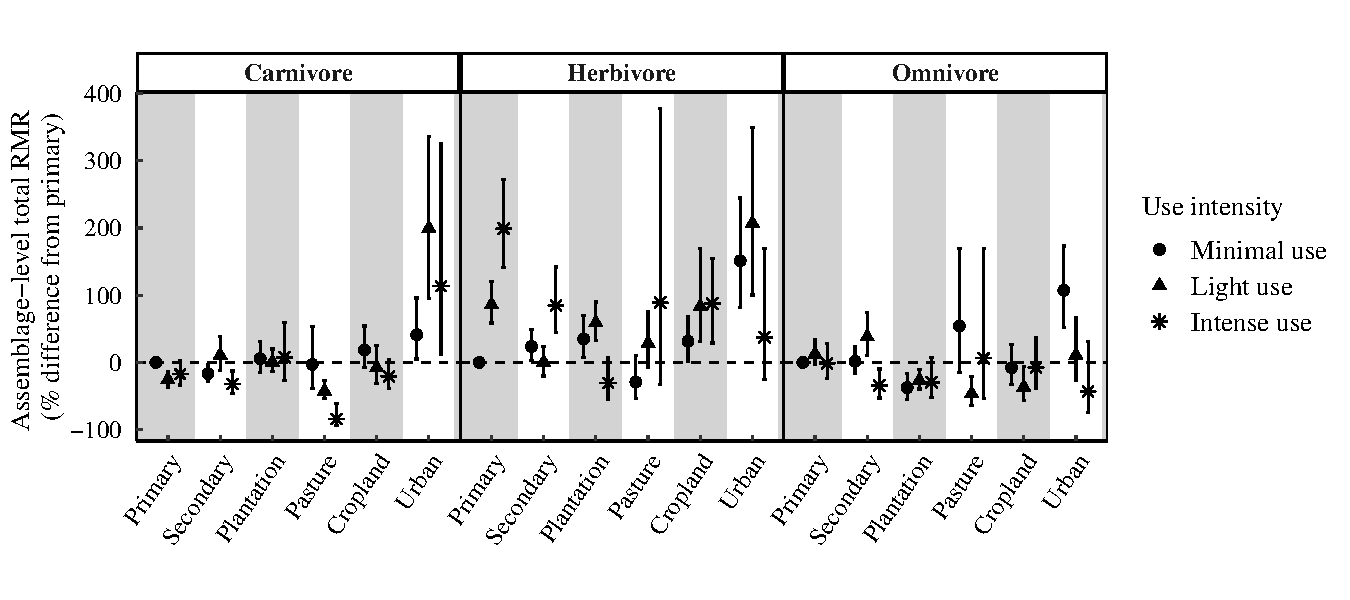
\includegraphics[scale=0.75]{figures/Chapter5/Figure3}
\caption[Effects of land use, land-use intensity and trophic group on assemblage-level total RMR.]{\textbf{Effects of land use, land-use intensity and trophic group on assemblage-level total RMR.} Model predictions are rescaled with reference to minimally-used primary vegetation, considered to be the undisturbed baseline. Primary: primary vegetation; secondary: secondary vegetation; plantation: plantation forest. }
\label{chap5_fig3}
\end{figure}


\subsection{Effects of land use, land-use intensity, trophic group and residual RMR on species’ occurrence probability}

Species’ occurrence probability was significantly affected by land use, land-use intensity, trophic level, residual RMR and their interactions (Figures \ref{chap5_fig4}, \ref{chap5_fig5}). Contrary to our expectations, species with higher residual RMR (relative to their body mass and taxonomic position) tended to do better than species with lower residual RMR in a number of disturbed land uses. Overall, land-use type was more important for determining the relationship between occurrence probability and residual RMR than land-use intensity (Figure \ref{chap5_fig4}a).

For minimally-used primary vegetation (reference), the model predicted negative effects of residual RMR on species occurrence probability in all trophic levels (but with a significant slope for herbivores only; Figure \ref{chap5_fig4}a). However, the directionality of this relationship was reversed in some disturbed land uses in all trophic groups (secondary vegetation, cropland and urban for omnivores; cropland for herbivores; urban for carnivores), with significant positive slopes, also significantly higher than those observed for primary vegetation (Figure \ref{chap5_fig4}a). The only exception was the opposite pattern for urban herbivores (\ref{chap5_fig4}b), where residual RMR had a more negative effect on occurrence probability than in minimally-used primary vegetation.
 
%% Figure 
\begin{figure}[h!]
\centering
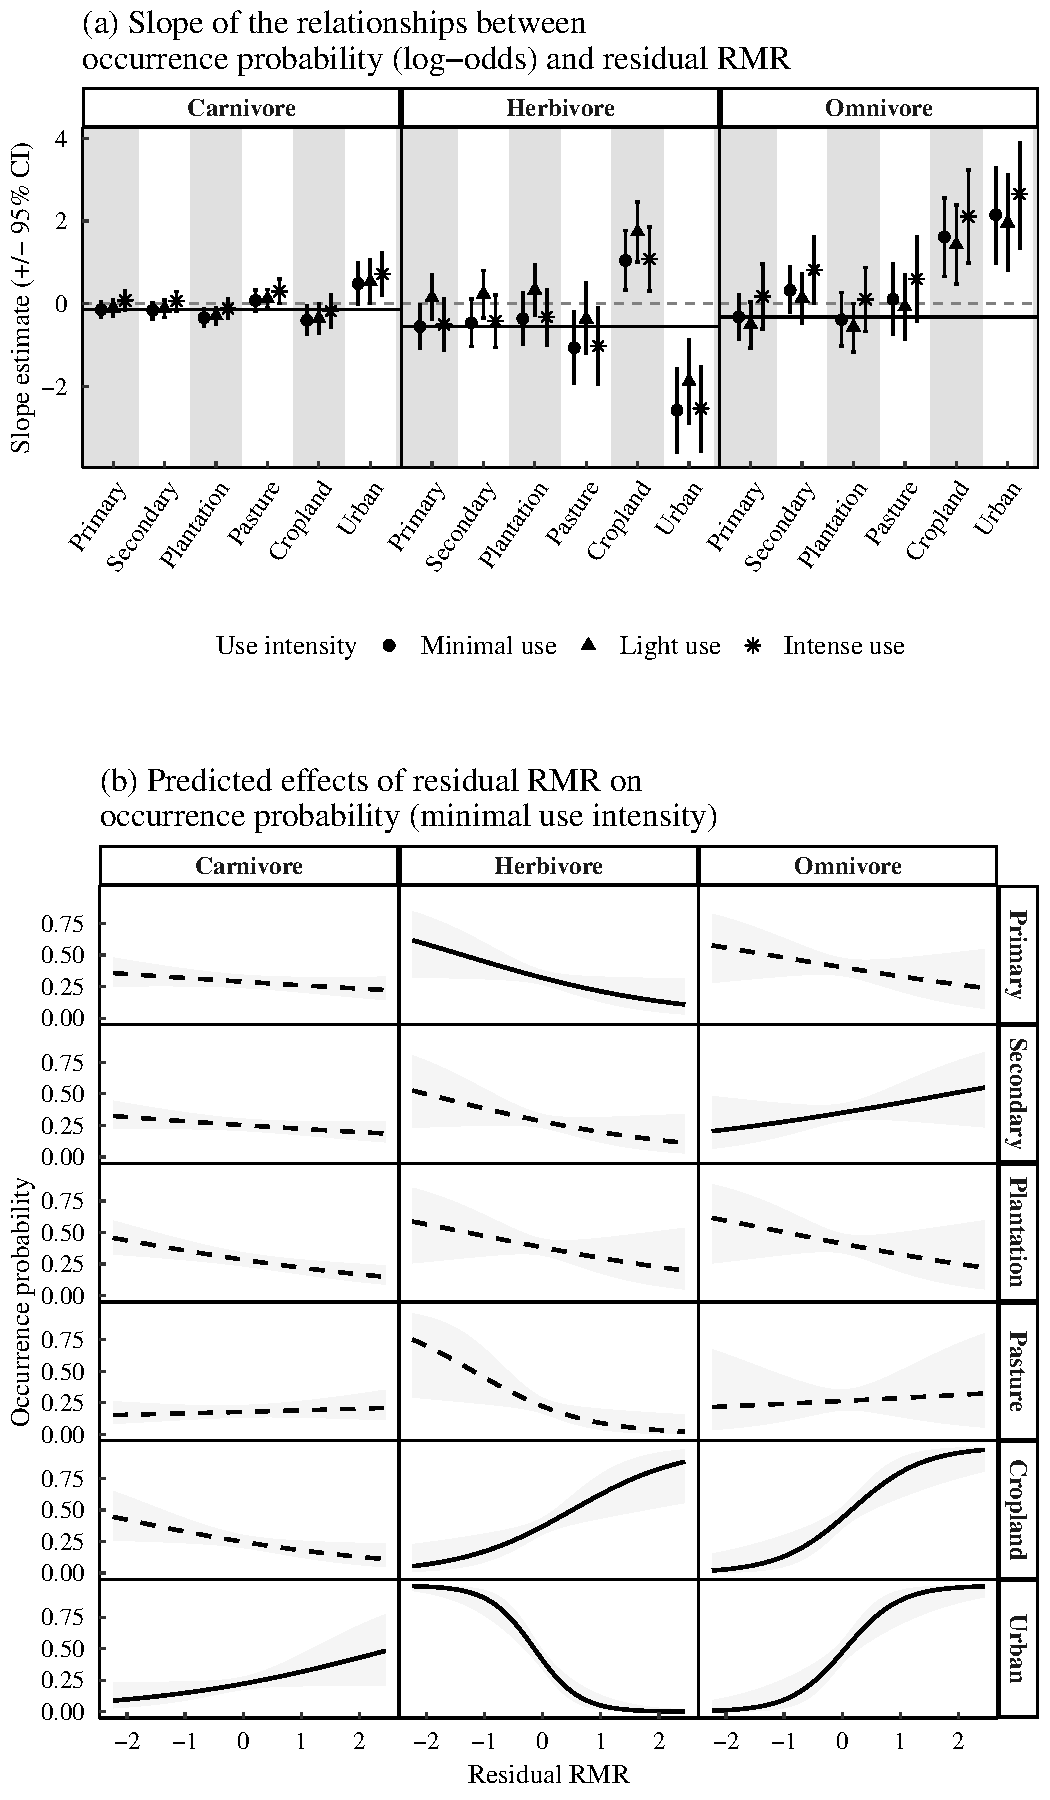
\includegraphics[scale=0.65]{figures/Chapter5/Figure4}
\caption[Slope estimates and predictions for the relationship between occurrence probability and residual RMR]{\textbf{(a) Slope estimates for the relationship between residual RMR and occurrence probability in each land-use type and for the three levels of land-use intensity.} The black horizontal line indicates the slope for the reference level (primary vegetation) for minimal land-use intensity. The grey dashed line marks 0. Error bars are 95\% confidence intervals. \textbf{(b) Effect of residual RMR on species probability of occurrence within each trophic level and for each land use-type.} I plotted the predictions for minimal land-use intensity only. Solid lines represent significant relationships. Primary: primary vegetation; secondary: secondary vegetation; plantation: plantation forest.}
\label{chap5_fig4}
\end{figure}

\clearpage 
I would like to emphasize that positive effects of residual RMR on occurrence probability in some of the most disturbed land uses (e.g., urban for carnivores) do not mean that there were absolute increases in species occurrence probability in disturbed land uses compared to primary vegetation (and vice-versa). I illustrate this point in Figure \ref{chap5_fig5}. For carnivores with a median value for residual RMR, occurrence probability was reduced by an average 24\% in urban land uses compared to primary vegetation. 

%% Figure 
\begin{figure}[h!]
\centering
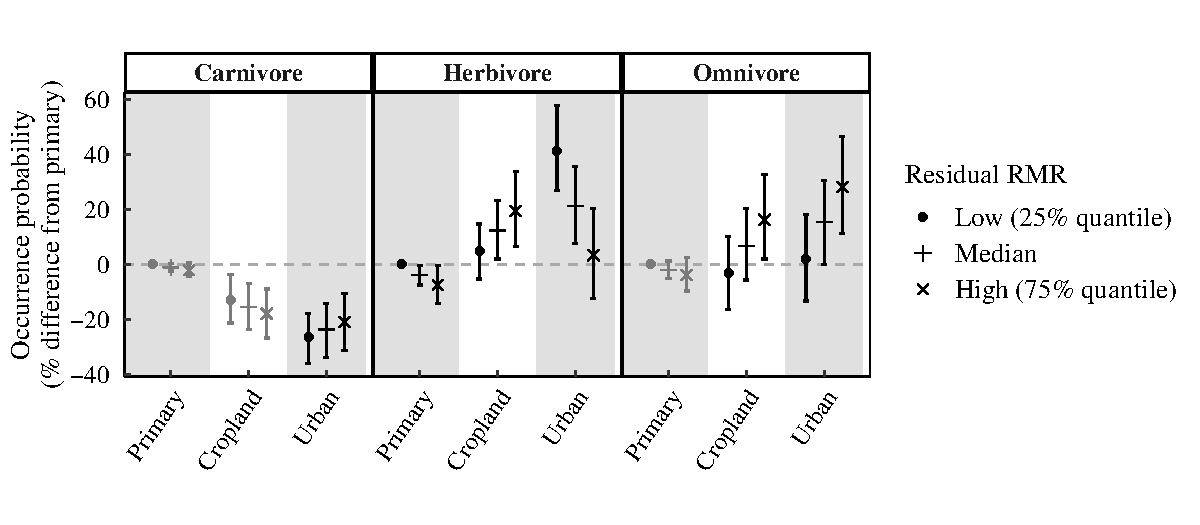
\includegraphics[scale=0.65]{figures/Chapter5/Figure5}
\caption[Predicted occurrence probabilities in primary vegetation and for the most disturbed land uses where residual RMR was found to have a significant effect on occurrence probability]{\textbf{Predicted occurrence probabilities (+/- 95\% confidence interval) in primary vegetation (primary) and for the most disturbed land uses where residual RMR was found to have a significant effect on occurrence probability.} For visualisation purposes, I discretised residual RMR in three levels. The predicted probabilities of occurrence were rescaled with reference to primary vegetation for the lowest value of residual RMR (25\% quantile). Here, the predictions are plotted for minimal land-use intensity (effects would be similar for light and intense land-use intensities). Black points and error bars are plotted where the relationship between occurrence probability and residual RMR was significant (and dark grey points and error bars represent non-significant trends).}
\label{chap5_fig5}
\end{figure}

Finally, the model showed some degree of deviation from distributional assumptions (diagnostic plots, Fig. S6). Nevertheless, the model's coefficients were similar when estimated with a Bayesian framework, suggesting that the estimates were robust (Fig. S7). The phylogenetic signal in the model residuals was weak and non-significant ($\lambda$=0.004, P=0.24). Re-fitting the model using the complete data subset (i.e., excluding imputed RMR estimates) showed that our conclusions are likely robust to imputation uncertainty (Fig. S8), with congruent results overall, although there were a few differences in the predictions between the two models – notably, for herbivores in urban land uses (Fig. S8).  


\clearpage
\section{Discussion}
